

Stochastic variables are foundational to understanding system reliability and risk assessment. They represent quantities subject to randomness, varying in value according to inherent uncertainties or natural variations. Probability distributions quantitatively describe this randomness, allocating probabilities across the range of possible values a stochastic variable can take.

\subsection*{Probability Models}
Probability models are mathematical representations of random phenomena. They are crucial for predicting the likelihood of various outcomes within a given set of conditions. In system reliability, these models help estimate the probability of system failures and assess potential risks.

\subsection*{Stochastic Variables}
\begin{itemize}
    \item \textbf{Definition}: A stochastic variable, $X$, is a variable whose value is subject to variations due to randomness. The concept is a cornerstone of probability theory and essential in engineering for modeling uncertainties.
    \item \textbf{Continuous vs. Discrete}: Stochastic variables can be continuous, taking any value within a range, or discrete, assuming specific isolated values. This distinction influences the choice of probability distribution to model the variable.
\end{itemize}

\subsection*{Probability Distribution Functions}
A probability distribution assigns a probability to each possible value of a stochastic variable. Various functions can describe the distribution, each providing different insights into the variable's behavior.

\begin{itemize}
    \item \textbf{Probability Density Function (PDF)}, $f(x)$:\\ Describes the probability density at each point for continuous variables. It's defined mathematically as $f(x) = \frac{d}{dx}F(x)$.

        The PDF is particularly useful in finding the likelihood of a specific outcome. For instance, in engineering, understanding the distribution of stress or load on a material can be achieved through the PDF, aiding in designing more robust structures.

    
    \item \textbf{Cumulative Distribution Function (CDF)}, $F(x)$:\\Gives the probability that the variable is less than or equal to a value, mathematically expressed as $F(x) = P(X \leq x)$.

    The CDF determines the probability of a variable falling within a particular range. This is especially useful in project scheduling, where it estimates the likelihood of completing a task by a certain deadline, thereby assisting in effective project management.

    
    \item \textbf{Complementary Cumulative Distribution Function (CCDF)}, $\bar{F}(x)$:\\ Shows the probability of the variable being greater than a specific value, denoted as $\bar{F}(x) = 1 - F(x)$.

    The CCDF is helpful when the tail or head of the distribution is being studied, making it a valuable tool in reliability engineering and survival analysis. Understanding the tails of distributions allows engineers and analysts to assess the risk of rare but impactful events, such as extreme loads or stresses that could lead to failure.

\end{itemize}

\begin{figure}[ht]
\centering
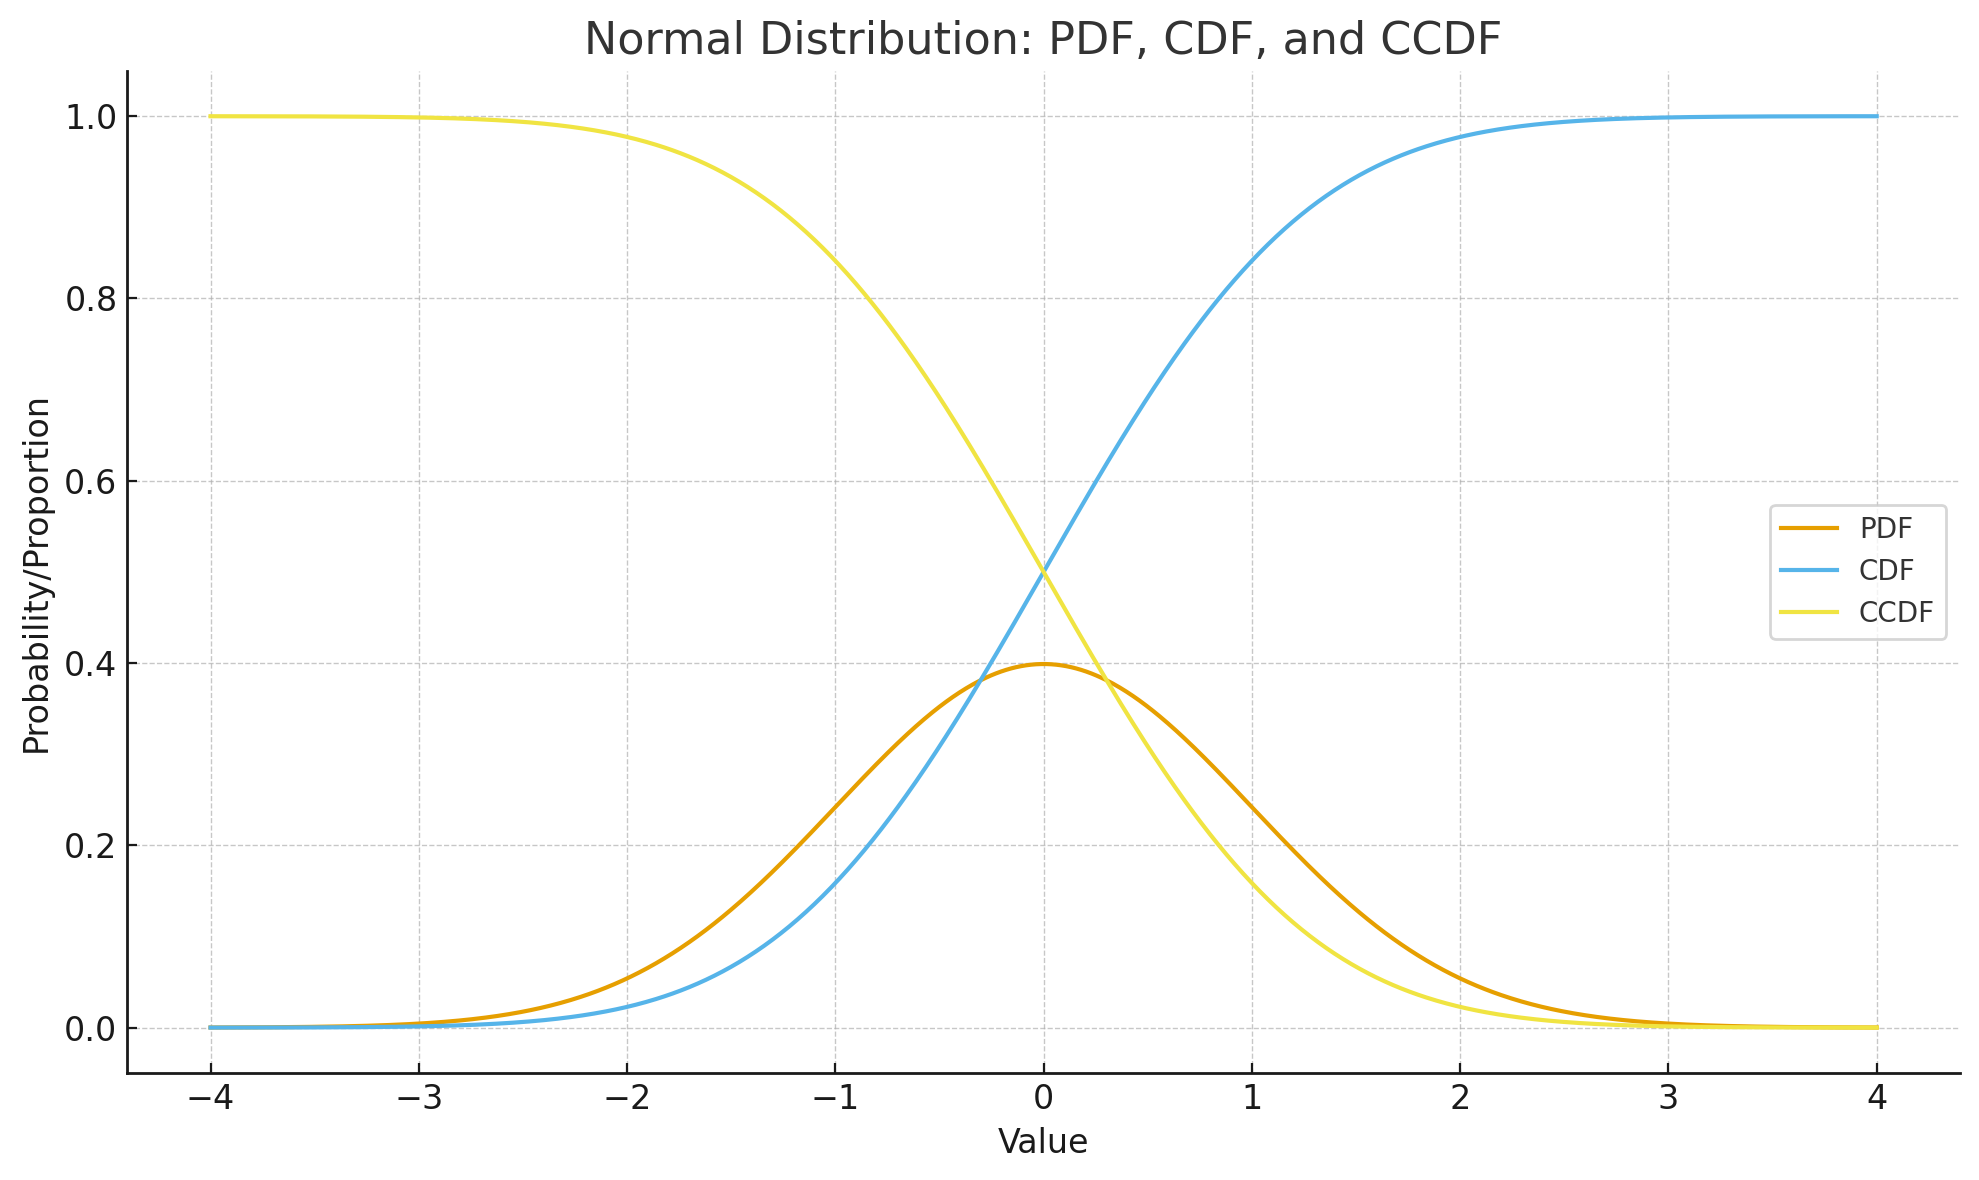
\includegraphics[width=0.8\linewidth]{figures/cdf.png}
\caption{Illustration of the Probability Density Function (PDF), Cumulative Distribution Function (CDF), and Complementary Cumulative Distribution Function (CCDF) for a standard normal distribution. }
\label{fig:distributions}
\end{figure}

\subsection*{Characteristics of Stochastic Variables}
These characteristics provide summary measures of the distribution's shape and spread, offering insights into the variable's behavior.

\begin{itemize}
    \item \textbf{Mean (Expected Value)}: \( \mu = E[X] \), the average of all possible values, weighted by their probabilities.
    \item \textbf{Variance and Standard Deviation}: \( \sigma^2 = Var(X) \) and \( \sigma = \sqrt{Var(X)} \), measure the variability or spread of the distribution. The standard deviation is the square root of variance, providing a measure of dispersion in the same units as the variable.
    \item \textbf{Coefficient of Variation}: \( \frac{\sigma}{\mu} \), the ratio of the standard deviation to the mean, offering a normalized measure of dispersion.
\end{itemize}
\newpage
\subsection*{Did you know? - The Log Scale}
\begin{mdframed}[backgroundcolor=gray!20] 
Logarithmic scales are essential for compactly displaying data across a wide range of values, especially when dealing with multiplicative effects or variables spanning several orders of magnitude. They reveal patterns and relationships more effectively than linear scales, particularly in log-normal distributions in reliability engineering, where the CDF and PDF are applied to the variable's logarithm.
\end{mdframed} 

\subsection*{Assignment 1}
The first assignment delves into the practical application of these concepts, focusing on the scheduling of project activities modeled with stochastic variables.

Understanding the relationship between the PDF and CDF is crucial for this assignment. The PDF provides the probability density of a stochastic variable at a specific value, while the CDF accumulates these probabilities up to a given point. This interrelation is fundamental in determining the likelihood of completing project activities within their scheduled durations.

The assignment also introduces the importance of correctly applying probability operations. The rules of product and sum play a pivotal role in calculating the likelihood of sequential or simultaneous events.